\documentclass{article}
\usepackage[T1]{fontenc}

\usepackage{graphicx}
\usepackage{listings}
\begin{document}

\title{FOSS Lab Report}
\author{Gokul K\\[2\baselineskip]
Roll Number: 21\\[2\baselineskip]}
\date{02 February 2020}

\maketitle

\setcounter{section}{12}
\section{Shell Programming IX}
\subsection{Aim}
Write a shell script which receives two file names as arguments. It
should check whether the two file contents are same or not. If they are
same then second file should be deleted.


\subsection{Source Code}
\begin{verbatim}
    #! /bin/bash

    # Gokul K
    # Roll No: 21
    # 25-01-2020

    # Write a shell script which receives two file names as arguments. It
    # should check whether the two file contents are same or not. If they are
    # same then second file should be deleted.

    if [[ $# -ne 2 ]]
    then
        echo "Invalid number of arguments"
        exit
    fi

    if [[ !(-f $1) || !(-f $2) ]]
    then
        echo "Enter valid filenames"
        exit
    fi

    text="`diff $1 $2 | wc -l`"

    if [[ text -eq 0 ]]
    then
        echo "Both files are the same. Removing $2"
        rm $2
        exit
    else
        echo "Both files are different"
        exit
    fi
\end{verbatim}

\subsection{Program Description}
Here the two files given as input is compared using diff command. if
diff command returns empty string, then the files can be safely assumed
as identical and the second file is removed.

\subsection{Output}
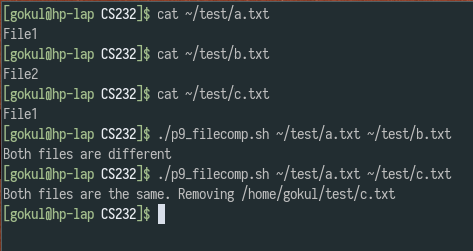
\includegraphics[width=0.9\textwidth]{img/p13.png}\newline

\subsection{Result}
The above program is run on Manjaro Linux shell. The file given as the second
output was removed if it was as same as the first.
\end{document}